\chapter{Getting started}
\label{getting-started}


\section{Let's run a regression}
\label{starting-regression}

This introduction is mostly angled towards the graphical client
program; please see Chapter~\ref{cli} below and the \emph{Gretl Command
  Reference} for details on the command-line program, \app{gretlcli}.
    
You can supply the name of a data file to open as an argument to
\app{gretl}, but for the moment let's not do that: just fire up the
program.\footnote{For convenience I will refer to the graphical client
  program simply as \app{gretl} in this manual. Note, however, that
  the specific name of the program differs according to the computer
  platform.  On Linux it is called \verb+gretl_x11+ while on MS
  Windows it is \verb+gretlw32.exe+. On Linux systems a wrapper script
  named \verb+gretl+ is also installed --- see also the \GCR.}  You
should see a main window (which will hold information on the data set
but which is at first blank) and various menus, some of them disabled
at first.
    
What can you do at this point?  You can browse the supplied data files
(or databases), open a data file, create a new data file, read the
help items, or open a command script.  For now let's browse the
supplied data files.  Under the File menu choose ``Open data, Sample
file''.  A second notebook-type window will open, presenting the sets
of data files supplied with the package (see
Figure~\ref{fig-datafiles}).  Select the first tab, ``Ramanathan''.
The numbering of the files in this section corresponds to the chapter
organization of Ramanathan (2002), which contains discussion of the
analysis of these data. The data will be useful for practice purposes
even without the text.
    
\begin{figure}[htbp]
  \begin{center}
    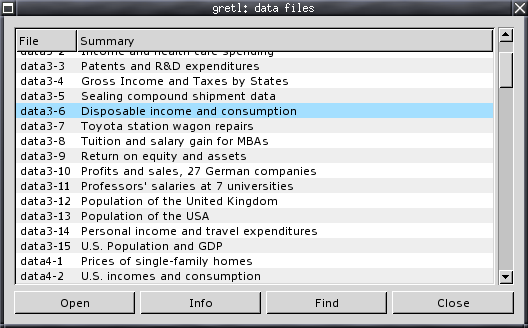
\includegraphics[scale=0.5]{figures/datafiles}
  \end{center}
  \caption{Practice data files window}
  \label{fig-datafiles}
\end{figure}

If you select a row in this window and click on ``Info'' this opens a
window showing information on the data set in question (for example,
on the sources and definitions of the variables).  If you find a file
that is of interest, you may open it by clicking on ``Open'', or just
double-clicking on the file name. For the moment let's open
\verb+data3-6+.  

\tip{In \app{gretl} windows containing lists, double-clicking on a
  line launches a default action for the associated list entry: e.g.\
  displaying the values of a data series, opening a file.}

This file contains data pertaining to a classic
econometric ``chestnut'', the consumption function.  The data window
should now display the name of the current data file, the overall data
range and sample range, and the names of the variables along with
brief descriptive tags --- see Figure~\ref{fig-mainwin}.
    
\begin{figure}[htbp]
  \begin{center}
    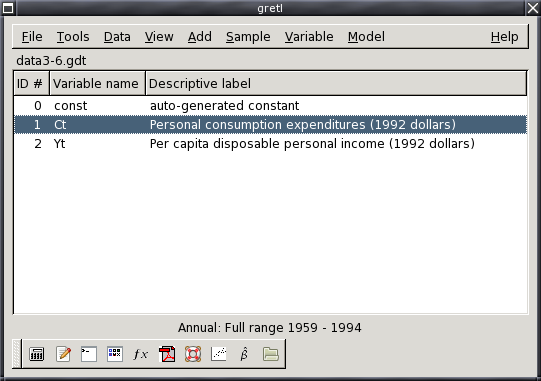
\includegraphics[scale=0.5]{figures/mainwin}
  \end{center}
  \caption{Main window, with a practice data file open}
  \label{fig-mainwin}
\end{figure}

OK, what can we do now?  Hopefully the various menu options should be
fairly self explanatory.  For now we'll dip into the Model menu; a
brief tour of all the main window menus is given in
Section~\ref{menus} below.
    
\app{gretl}'s Model menu offers numerous various econometric
estimation routines.  The simplest and most standard is Ordinary Least
Squares (OLS). Selecting OLS pops up a dialog box calling for a
\emph{model specification} --- see Figure~\ref{fig-selector}.
    
\begin{figure}[htbp]
  \begin{center}
    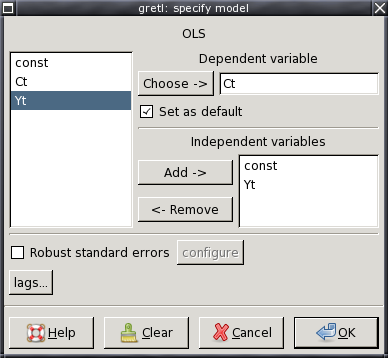
\includegraphics[scale=0.5]{figures/selector}
  \end{center}
  \caption{Model specification dialog}
  \label{fig-selector}
\end{figure}

To select the dependent variable, highlight the variable you want in
the list on the left and click the ``Choose'' button that points to
the Dependent variable slot.  If you check the ``Set as default'' box
this variable will be pre-selected as dependent when you next open the
model dialog box. Shortcut: double-clicking on a variable on the left
selects it as dependent and also sets it as the default. To select
independent variables, highlight them on the left and click the
``Add'' button (or click the right mouse button over the highlighted
variable).  To select several variable in the list box, drag the mouse
over them; to select several non-contiguous variables, hold down the
\verb+Ctrl+ key and click on the variables you want.  To run a
regression with consumption as the dependent variable and income as
independent, click \verb+Ct+ into the Dependent slot and add \verb+Yt+
to the Independent variables list.


\section{Estimation output}
\label{est-output}

Once you've specified a model, a window displaying the regression
output will appear.  The output is reasonably comprehensive and in a
standard format (Figure~\ref{fig-modelwin}).
    
\begin{figure}[htbp]
  \begin{center}
    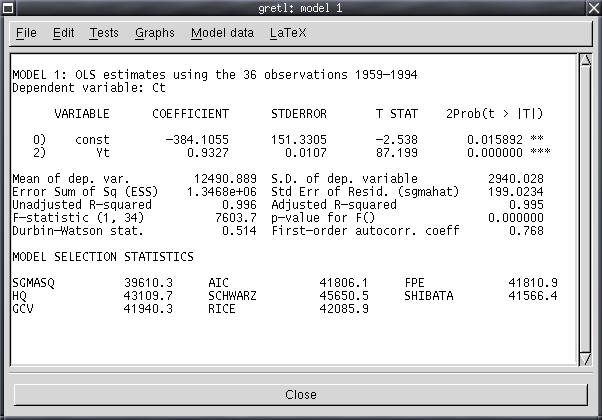
\includegraphics[scale=0.5]{figures/modelwin}
  \end{center}
  \caption{Model output window}
  \label{fig-modelwin}
\end{figure}

The output window contains menus that allow you to inspect or graph
the residuals and fitted values, and to run various diagnostic tests
on the model. 

For most models there is also an option to print the regression
output in {\LaTeX} format.  See Chapter~\ref{gretltex} for details.

To import \app{gretl} output into a word processor, you may copy and
paste from an output window, using its \textsf{Edit} menu (or Copy
button, in some contexts) to the target program.  Many (not all)
\app{gretl} windows offer the option of copying in RTF (Microsoft's
``Rich Text Format'') or as {\LaTeX}. If you are pasting into a word
processor, RTF may be a good option because the tabular formatting of
the output is preserved.\footnote{Note that when you copy as RTF under
  MS Windows, Windows will only allow you to paste the material into
  applications that ``understand'' RTF.  Thus you will be able to
  paste into MS Word, but not into notepad.  Note also that there
  appears to be a bug in some versions of Windows, whereby the paste
  will not work properly unless the ``target'' application (e.g.\  MS
  Word) is already running prior to copying the material in question.}
Alternatively, you can save the output to a (plain text) file then
import the file into the target program.  When you finish a
\app{gretl} session you are given the option of saving all the output
from the session to a single file.

 Note that on the \app{gnome} desktop and under MS Windows, the
 \textsf{File} menu includes a command to send the output directly to
 a printer.

 \tip{When pasting or importing plain text \app{gretl} output into a
   word processor, select a monospaced or typewriter-style font (e.g.\
   Courier) to preserve the output's tabular formatting.  Select a
   small font (10-point Courier should do) to prevent the output lines
   from being broken in the wrong place.}

\section{The main window menus}
\label{menus}

Reading left to right along the main window's menu bar, we find the
File, Tools, Data, View, Add, Sample, Variable, Model and Help menus.

\begin{center}
  
\includegraphics[scale=0.75]{figures/menubar}
\end{center}

\begin{itemize}
\item \textsf{File menu}
  \begin{itemize}
  \item \textsf{Open data}: Open a native \app{gretl} data file or
    import from other formats.  See Chapter~\ref{datafiles}.
  \item \textsf{Append data}: Add data to the current working data
    set, from a \app{gretl} data file, a comma-separated values file
    or a spreadsheet file.
  \item \textsf{Save data}: Save the currently open native \app{gretl}
    data file.
  \item \textsf{Save data as}: Write out the current data set in
    native format, with the option of using gzip data compression. See
    Chapter~\ref{datafiles}.
  \item \textsf{Export data}: Write out the current data set in Comma
    Separated Values (CSV) format, or the formats of GNU R or GNU
    Octave. See Chapter~\ref{datafiles} and also
    Appendix~\ref{app-advanced}.
  \item \textsf{Send to}: Send the current data set as an e-mail
    attachment.
  \item \textsf{New data set}: Allows you to create a blank data set,
    ready for typing in values or for importing series from a
    database.  See below for more on databases.
  \item \textsf{Clear data set}: Clear the current data set out of
    memory.  Generally you don't have to do this (since opening a new
    data file automatically clears the old one) but sometimes it's
    useful.
  \item \textsf{Script files}: A ``script'' is a file containing a
    sequence of \app{gretl} commands.  This item contains entries
    that let you open a script you have created previously (``User
    file''), open a sample script, or open an editor window in which
    you can create a new script.
  \item \textsf{Session files}: A ``session'' file contains a snapshot
    of a previous \app{gretl} session, including the data set used
    and any models or graphs that you saved.  Under this item you
    can open a saved session or save the current session.
  \item \textsf{Databases}: Allows you to browse various large
    databases, either on your own computer or, if you are connected
    to the internet, on the \app{gretl} database server.  See
    Section~\ref{dbase} for details.
  \item \textsf{Function files}: Handles ``function packages'' (see
    Section~\ref{sec:func-packages}), which allow you to access
    functions written by other users and share the ones written by
    you.
  \item \textsf{Exit}: Quit the program. If expert mode is not
    selected you'll be prompted to save any unsaved work.
  \end{itemize}

\item \textsf{Tools menu}
  \begin{itemize}
  \item \textsf{Statistical tables}: Look up critical values for
    commonly used distributions (normal or Gaussian, \emph{t},
    chi-square, \emph{F} and Durbin--Watson).
  \item \textsf{P-value finder}: Open a window which enables you to
    look up p-values from the Gaussian, \emph{t}, chi-square,
    \emph{F}, gamma or binomial distributions. See also the
    \cmd{pvalue} command in the \emph{Gretl Command Reference}.
  \item \textsf{Test statistic calculator}: Calculate test statistics
    and p-values for a range of common hypothesis tests (population
    mean, variance and proportion; difference of means, variances and
    proportions).  See also the item ``Bivariate tests'' under the
    Model menu.
  \item \textsf{Command log}: Open a window containing a record
    of the commands executed so far.
  \item \textsf{Gretl console}: Open a ``console'' window into which
    you can type commands as you would using the command-line program,
    \app{gretlcli} (as opposed to using point-and-click).
  \item \textsf{Start Gnu R}: Start \app{R} (if it is installed on
    your system), and load a copy of the data set currently open in
    \app{gretl}.  See Appendix~\ref{app-advanced}.
  \item \textsf{Sort variables}: Rearrange the listing of variables in
    the main window, either by ID number or alphabetically by name.
  \item \textsf{NIST test suite}: Check the numerical accuracy of
    \app{gretl} against the reference results for linear regression
    made available by the (US) National Institute of Standards and
    Technology.
  \item \textsf{Preferences}: Set the paths to various files
    \app{gretl} needs to access. Choose the font in which gretl
    displays text output.  Select or unselect ``expert mode''. (If
    this mode is selected various warning messages are suppressed.)
    Activate or suppress \app{gretl}'s messaging about the
    availability of program updates.  Configure or turn on/off the
    main-window toolbar. See the \GCR\ for
    further details.
  \end{itemize}

\item \textsf{Data menu}
  \begin{itemize}
  \item \textsf{Select all}: Several menu items act upon those
    variables that are currently selected in the main window.  This
    item lets you select all the variables.
  \item \textsf{Display values}: Pops up a window with a simple (not
    editable) printout of the values of the selected variable or
    variables.
  \item \textsf{Edit values}: Opens a spreadsheet window where you
    can edit the values of the selected variables. 
  \item \textsf{Add observations}: Gives a dialog box in which you can
    choose a number of observations to add at the end of the current
    dataset; for use with forecasting.
  \item \textsf{Remove extra observations}: Active only if extra
    observations have been added automatically in the process of
    forecasting; deletes these extra observations.
  \item \textsf{Read info}, \textsf{Edit info}: ``Read info'' just
    displays the summary information for the current data file; ``Edit
    info'' allows you to make changes to it (if you have permission to
    do so).
  \item \textsf{Print description}: Opens a window containing a full
    account of the current dataset, including the summary information
    and any specific information on each of the variables.
  \item \textsf{Add case markers}: Prompts for the name of a text file
    containing ``case markers'' (short strings identifying the
    individual observations) and adds this information to the data
    set. See Chapter~\ref{datafiles}.
  \item \textsf{Remove case markers}: Active only if the dataset has
    case markers identifying the observations; removes these case
    markers.
  \item \textsf{Dataset structure}: invokes a series of dialog boxes
    which allow you to change the structural interpretation of the
    current dataset.  For example, if data were read in as a cross
    section you can get the program to interpret them as time series
    or as a panel.  See also section~\ref{sec:data-structure}.
  \item \textsf{Compact data}: For time-series data of higher than
    annual frequency, gives you the option of compacting the data to a
    lower frequency, using one of four compaction methods (average,
    sum, start of period or end of period).
  \item \textsf{Expand data}: For time-series data, gives you the
    option of expanding the data to a higher frequency.
  \item \textsf{Transpose data}: Turn each observation into a variable
    and vice versa (or in other words, each row of the data matrix
    becomes a column in the modified data matrix); can be useful with
    imported data that have been read in ``sideways''.
  \end{itemize}

\item \textsf{View menu} 
  \begin{itemize}
  \item \textsf{Icon view}: Opens a window showing the content of
    the current session as a set of icons; see section~\ref{session}.
  \item \textsf{Graph specified vars}: Gives a choice between a time
    series plot, a regular X--Y scatter plot, an X--Y plot using
    impulses (vertical bars), an X--Y plot ``with factor separation''
    (i.e.\ with the points colored differently depending to the value
    of a given dummy variable), boxplots, and a 3-D graph. Serves up a
    dialog box where you specify the variables to graph. See
    Chapter~\ref{chap-graphs} for details.
  \item \textsf{Multiple graphs}: Allows you to compose a set of up to
    six small graphs, either pairwise scatter-plots or time-series
    graphs.  These are displayed together in a single window.
  \item \textsf{Summary statistics}: Shows a full set of
    descriptive statistics for the variables selected in the main
    window.
  \item \textsf{Correlation matrix}: Active only if two or more
    variables are selected; shows the pairwise correlation
    coefficients for the selected variables.
  \item \textsf{Principal components}: Active only if two or more
    variables are selected; produces a Principal Components Analysis
    of the selected variables.
  \item \textsf{Mahalonobis distances}: Active only if two or more
    variables are selected; computes the Mahalonobis distance of each
    observation from the centroid of the selected set of variables.
  \end{itemize}

\item \textsf{Add menu} Offers various standard transformations
  of variables (logs, lags, squares, etc.) that you may wish to add to
  the data set. Also gives the option of adding random variables, and
  (for time-series data) adding seasonal dummy variables (e.g.\
  quarterly dummy variables for quarterly data).

\item \textsf{Sample menu}
  \begin{itemize}
  \item \textsf{Set range}: Select a different starting and/or ending
    point for the current sample, within the range of data available.
  \item \textsf{Restore full range}: self-explanatory.
  \item \textsf{Define, based on dummy}: Given a dummy (indicator)
    variable with values 0 or 1, this drops from the current sample
    all observations for which the dummy variable has value 0.
  \item \textsf{Restrict, based on criterion}: Similar to the item
    above, except that you don't need a pre-defined variable: you
    supply a Boolean expression (e.g.\ \verb+sqft > 1400+) and the
    sample is restricted to observations satisfying that condition.
    See the entry for \cmd{genr} in the \GCR\
    for details on the Boolean operators that can be used.
  \item \textsf{Random sub-sample}: Draw a random sample from the full dataset.
  \item \textsf{Drop all obs with missing values}: Drop from the
    current sample all observations for which at least one variable
    has a missing value (see Section~\ref{missing-data}).
  \item \textsf{Count missing values}: Give a report on observations
    where data values are missing. May be useful in examining a panel
    data set, where it's quite common to encounter missing values.
  \item \textsf{Set missing value code}: Set a numerical value that
    will be interpreted as ``missing'' or ``not available''.  This is
    intended for use with imported data, when \app{gretl} has not
    recognized the missing-value code used.
  \end{itemize}

\item \textsf{Variable menu} Most items under here operate on a single
  variable at a time.  The ``active'' variable is set by highlighting
  it (clicking on its row) in the main data window.  Most options will
  be self-explanatory.  Note that you can rename a variable and can
  edit its descriptive label under ``Edit attributes''. You can also
  ``Define a new variable'' via a formula (e.g.\ involving some
  function of one or more existing variables). For the syntax of such
  formulae, look at the online help for ``Generate variable syntax''
  or see the \cmd{genr} command in the \emph{Gretl Command Reference}.
  One simple example:
          
\begin{code} 
foo = x1 * x2
\end{code}

  will create a new variable \verb+foo+ as the product of the existing
  variables \verb+x1+ and \verb+x2+.  In these formulae, variables
  must be referenced by name, not number.

\item \textsf{Model menu} For details on the various estimators
  offered under this menu please consult the \emph{Gretl Command
    Reference}.  Also see Chapter~\ref{chap-nls} regarding the
  estimation of nonlinear models.

\item \textsf{Help menu} Please use this as needed! It gives details
  on the syntax required in various dialog entries.
\end{itemize}


\section{Keyboard shortcuts}
\label{keyb-accel}

When working in the main \app{gretl} window, some common operations
may be performed using the keyboard, as shown in the table below.

\begin{center}
\begin{tabular}{lp{5in}}
  \texttt{Return} & Opens a window displaying the values of the currently
  selected variables: it is the same as selecting ``Data, Display
  Values''. \\
  \texttt{Delete} & Pressing this key has the effect of deleting the
  selected variables. A confirmation is required, to prevent
  accidental deletions. \\
  \texttt{e} & Has the same effect as selecting ``Edit
  attributes'' from the ``Variable'' menu. \\
  \texttt{F2} & Same as ``e''. Included for compatibility with other
  programs.\\
  \texttt{g} & Has the same effect as selecting ``Define new
  variable'' from the ``Variable'' menu (which maps onto the
  \texttt{genr} command).\\
  \texttt{h} & Opens a help window for gretl commands.\\
  \texttt{F1} & Same as ``h''. Included for compatibility with other
  programs.\\
  \texttt{r} & Refreshes the variable list in the main window: has 
  the same effect as selecting ``Refresh window'' from the ``Data'' menu. \\
  \texttt{t} & Graphs the selected variable; a line graph is used for
  time-series datasets, whereas a distribution plot is used for
  cross-sectional data. 
\end{tabular}
\end{center}

\section{The gretl toolbar}
\label{toolbar}

At the bottom left of the main window sits the toolbar.

\begin{center}
  
\includegraphics[scale=0.75]{figures/toolbar}
\end{center}

The icons have the following functions, reading from left to right:

\begin{enumerate}
\item Launch a calculator program.  A convenience function in case you
  want quick access to a calculator when you're working in
  \app{gretl}.  The default program is \verb+calc.exe+ under MS
  Windows, or \verb+xcalc+ under the X window system.  You can change
  the program under the ``Tools, Preferences, General'' menu,
  ``Programs'' tab.
\item Start a new script.  Opens an editor window in which you can
  type a series of commands to be sent to the program as a batch.
\item Open the gretl console.  A shortcut to the ``Gretl console''
  menu item (Section~\ref{menus} above).
\item Open the \app{gretl} session icon window.
\item Open the \app{gretl} website in your web browser.  This will
  work only if you are connected to the Internet and have a properly
  configured browser.
\item Open this manual in PDF format.
\item Open the help item for script commands syntax (i.e.\ a listing
  with details of all available commands).
\item Open the dialog box for defining a graph.
\item Open the dialog box for estimating a model using ordinary least
  squares.
\item Open a window listing the sample datasets supplied with
  \app{gretl}, and any other data file collections that have been
  installed.
\end{enumerate}

If you don't care to have the toolbar displayed, you can turn it off
under the ``Tools, Preferences, General'' menu. Go o the Toolbar tab
and uncheck the ``show gretl toolbar'' box.

%%% Local Variables: 
%%% mode: latex
%%% TeX-master: "gretl-guide"
%%% End: 

